%%%%%%%%%%%%%%%%%%%%%%%%%%%%%%%%%%%%%%%%%%%%%%%%%%%%%%%%%%%%%%%%%%%%%%%%%%%%%%%%

\begin{frame}{Bits of your ISA you need to describe}

\begin{itemize}
    \item Target machine
    \begin{itemize}
        \item Registers, register classes
        \item Calling conventions
    \end{itemize}
    \item Instruction set
    \begin{itemize}
        \item Operands and patterns
        \item Assembly printing and/or instruction encoding
        \item Schedule (not part of this talk)
    \end{itemize}
    \item ...
\end{itemize}

\end{frame}

%%%%%%%%%%%%%%%%%%%%%%%%%%%%%%%%%%%%%%%%%%%%%%%%%%%%%%%%%%%%%%%%%%%%%%%%%%%%%%%%

\talksection{Describing the target machine}

\begin{frame}{TableGen}

\begin{itemize}
    \item C++-style syntax
    \item Different set of backends
    \begin{itemize}
        \item RegisterInfo, InstrInfo, AsmWriter, ...
    \end{itemize}
    \item TableGen backends generate .inc files
    \begin{itemize}
        \item Included by your C++ files
    \end{itemize}
    \item More information:
    \begin{itemize}
        \item \url{llvm.org/docs/TableGen/index.html}
        \item \url{llvm.org/docs/TableGen/BackEnds.html}
    \end{itemize}
\end{itemize}

\end{frame}

%%%%%%%%%%%%%%%%%%%%%%%%%%%%%%%%%%%%%%%%%%%%%%%%%%%%%%%%%%%%%%%%%%%%%%%%%%%%%%%%

\begin{frame}[fragile]{Describing registers with TableGen}

\begin{itemize}
    \item TableGen provides the 'Register' class
    \begin{itemize}
        \item Can use the 'HWEncoding' field for encodings
    \end{itemize}
    \item Referenced as “LEG::R0” in C++
\end{itemize}

\begin{codebox}
class LEGReg<bits<16> Enc, string n> : Register<n> {
  Let HWEncoding = Enc;
  let Namespace = "LEG";
}

def R0 : LEGReg< 0, "r0" >;
...
def SP : LEGReg< 10, "sp" >;
\end{codebox}
\codecaption{LEGRegisterInfo.td}

\end{frame}

%%%%%%%%%%%%%%%%%%%%%%%%%%%%%%%%%%%%%%%%%%%%%%%%%%%%%%%%%%%%%%%%%%%%%%%%%%%%%%%%

\begin{frame}[fragile]{Describing registers with TableGen}

\begin{itemize}
    \item Can automate trivial definitions
\end{itemize}

\begin{codebox}
foreach i = 0-9 in {
  def R#i : R<i, "r"#i>;
}
\end{codebox}
\codecaption{LEGRegisterInfo.td}

\begin{itemize}
    \item Group registers into register classes
\end{itemize}

\begin{codebox}
def GRRegs : RegisterClass<"LEG", [i32], 32,
  (add SP, (sequence "R%i", 0, 9))>;
\end{codebox}
\codecaption{LEGRegisterInfo.td}

\end{frame}

%%%%%%%%%%%%%%%%%%%%%%%%%%%%%%%%%%%%%%%%%%%%%%%%%%%%%%%%%%%%%%%%%%%%%%%%%%%%%%%%

\talksection{Describing the instruction set}

\begin{frame}{Describing instructions: Overview}

\begin{itemize}
    \item Let's start with a simple instruction: \texttt{ADDrr}
    \begin{itemize}
        \item Adds two registers together
    \end{itemize}
    \item We define it in lib/Target/LEG/LEGInstrInfo.td
    \item What we need to specify:
    \begin{itemize}
        \item Operands
        \item Assembly string
        \item Instruction pattern
    \end{itemize}
\end{itemize}

\end{frame}

%%%%%%%%%%%%%%%%%%%%%%%%%%%%%%%%%%%%%%%%%%%%%%%%%%%%%%%%%%%%%%%%%%%%%%%%%%%%%%%%

\begin{frame}[fragile]{Describing instructions: Operands}

\begin{itemize}
    \item List of definitions or outputs ('outs')
    \item List of uses or inputs ('ins')
    \item Operand class:
    \begin{itemize}
        \item Register class (e.g. GRRegs)
        \item Immediate (e.g. i32imm)
        \item More complex operands (e.g. reg + imm for load/store)
    \end{itemize}
\end{itemize}

\begin{codebox}[commandchars=\\\{\}]
def ADDrr : InstLEG<\codeempha{(outs GRRegs:$dst)},
                    \codeempha{(ins GRRegs:$src1, GRRegs:$src2)},
                    "add $dst, $src1, $src2",
                    [(set i32:$dst, (add i32:$src1, i32:$src2))]>;
\end{codebox}
\codecaption[-10.2ex]{LEGInstrInfo.td}

\vspace{5ex}
\begin{itemize}
    \item Result:
\end{itemize}
\examplebox[firstline=4,lastline=4,gobble=1]{ex1/ex1-mi.txt}

\end{frame}

%%%%%%%%%%%%%%%%%%%%%%%%%%%%%%%%%%%%%%%%%%%%%%%%%%%%%%%%%%%%%%%%%%%%%%%%%%%%%%%%

\begin{frame}[fragile]{Describing instructions: Selection Patterns}

\begin{itemize}
    \item Matches nodes in the SelectionDAG
    \begin{itemize}
        \item Nodes get turned into MachineInstrs during ISel
        \item If pattern is omitted, selection needs to be done in C++
    \end{itemize}
    \item Syntax:
    \begin{itemize}
        \item One pair of parenthesis defines one node
        \item Nodes have DAG operands, with 'MVT' type (e.g. i32)
        \item Map DAG operands to MI operands
    \end{itemize}
\end{itemize}

\begin{codebox}[commandchars=\\\{\}]
def ADDrr : InstLEG<(outs GRRegs:$dst),
                    (ins GRRegs:$src1, GRRegs:$src2),
                    "add $dst, $src1, $src2",
                    \codeempha{[(set i32:$dst, (add i32:$src1, i32:$src2))]}>;
\end{codebox}
\codecaption[-10.2ex]{LEGInstrInfo.td}

\vspace{5ex}
\begin{itemize}
    \item Result:
\end{itemize}
\examplebox[firstline=4,lastline=4,gobble=1]{ex1/ex1-mi.txt}

\end{frame}

%%%%%%%%%%%%%%%%%%%%%%%%%%%%%%%%%%%%%%%%%%%%%%%%%%%%%%%%%%%%%%%%%%%%%%%%%%%%%%%%

\begin{frame}[fragile]{Constants}

\begin{itemize}
    \item Using constants in IR produces errors at this point
    \item We need to specify how to generate ('materialize') constants
    \item For example, with a 'move' instruction
    \begin{itemize}
        \item E.g. MOVLO for 16-bit constants
    \end{itemize}
\end{itemize}

\begin{itemize}
    \item Example:
\end{itemize}
\examplebox[firstline=8,lastline=8,gobble=4]{ex2/ex2.ll}

\begin{itemize}
    \item Result:
\end{itemize}
\begin{codebox}
LLVM ERROR: Cannot select: 0x29d4350: i32 = Constant<2> [ID=2]
In function: main
\end{codebox}

\end{frame}

%%%%%%%%%%%%%%%%%%%%%%%%%%%%%%%%%%%%%%%%%%%%%%%%%%%%%%%%%%%%%%%%%%%%%%%%%%%%%%%%

\begin{frame}[fragile]{Constants}

\begin{itemize}
    \item Let's define this move instruction:
\end{itemize}

\begin{codebox}
def MOVLOi16 : InstLEG<(outs GRRegs:$dst),
                      (ins i32imm:$src),
                      "movw $dst, $src",
                      [(set i32:$dst, i32imm:$src)]> {
  let isMoveImm = 1;
}
\end{codebox}
\codecaption{LEGInstrInfo.td}

\begin{itemize}
    \item Example:
\end{itemize}
\examplebox[firstline=8,lastline=8,gobble=4]{ex2/ex2.ll}

\begin{itemize}
    \item Result:
\end{itemize}
\examplebox[firstline=6,lastline=7,gobble=1]{ex2/ex2-ADDrr-MOVLO-mi.txt}

\end{frame}

%%%%%%%%%%%%%%%%%%%%%%%%%%%%%%%%%%%%%%%%%%%%%%%%%%%%%%%%%%%%%%%%%%%%%%%%%%%%%%%%

\begin{frame}[fragile]{Constants}

\begin{itemize}
    \item What if the instruction accepts an immediate operand?
\end{itemize}

\begin{codebox}[commandchars=\\¬|]
def \codeempha¬LEGimm8| : Operand<i32>, ImmLeaf<i32, [{
  return Imm >= 0 && Imm < 256;
}]>;

def ADDri : InstLEG<(outs GRRegs:$dst),
                    (ins GRRegs:$src1, \codeempha¬i32imm|:$src2),
                    "add $dst, $src1, $src2",
                    [(set i32:$dst, (add i32:$src1, 
                                     \codeempha¬LEGimm8|:$src2))]>;
\end{codebox}
\codecaption{LEGInstrInfo.td}

\begin{itemize}
    \item Example:
\end{itemize}
\examplebox[firstline=8,lastline=8,gobble=4]{ex2/ex2.ll}

\begin{itemize}
    \item Result:
\end{itemize}
\examplebox[firstline=6,lastline=6,gobble=1]{ex2/ex2-ADDri-mi.txt}

\end{frame}

%%%%%%%%%%%%%%%%%%%%%%%%%%%%%%%%%%%%%%%%%%%%%%%%%%%%%%%%%%%%%%%%%%%%%%%%%%%%%%%%

\begin{frame}[fragile]{Matching multiple DAG nodes}

\begin{itemize}
    \item DAG nodes can be nested inside selection patterns
    \begin{itemize}
        \item The output of one node is the input of another
    \end{itemize}
    \item Allows operations to be combined
    \begin{itemize}
        \item Reduces the number of generated instructions
        \item Possibly improves performance or power consumption
    \end{itemize}
    \item Example: multiply and add instruction (ex3.ll)
\end{itemize}

\begin{codebox}[commandchars=\\\{\}]
def MLA : InstLEG<(outs GRRegs:$dst),
                  (ins GRRegs:$src1, GRRegs:$src2, GRRegs:$src3),
                  "mla $dst, $src1, $src2, $src3",
                  [(set i32:$dst,
                   \codeempha{(add \codeemphb{(mul i32:$src1, i32:$src2)}, i32:$src3))}]>;
\end{codebox}
\codecaption[-12.2ex]{LEGInstrInfo.td}

\end{frame}

%%%%%%%%%%%%%%%%%%%%%%%%%%%%%%%%%%%%%%%%%%%%%%%%%%%%%%%%%%%%%%%%%%%%%%%%%%%%%%%%

\begin{frame}[fragile]{Matching multiple DAG nodes}

% FIXME center image
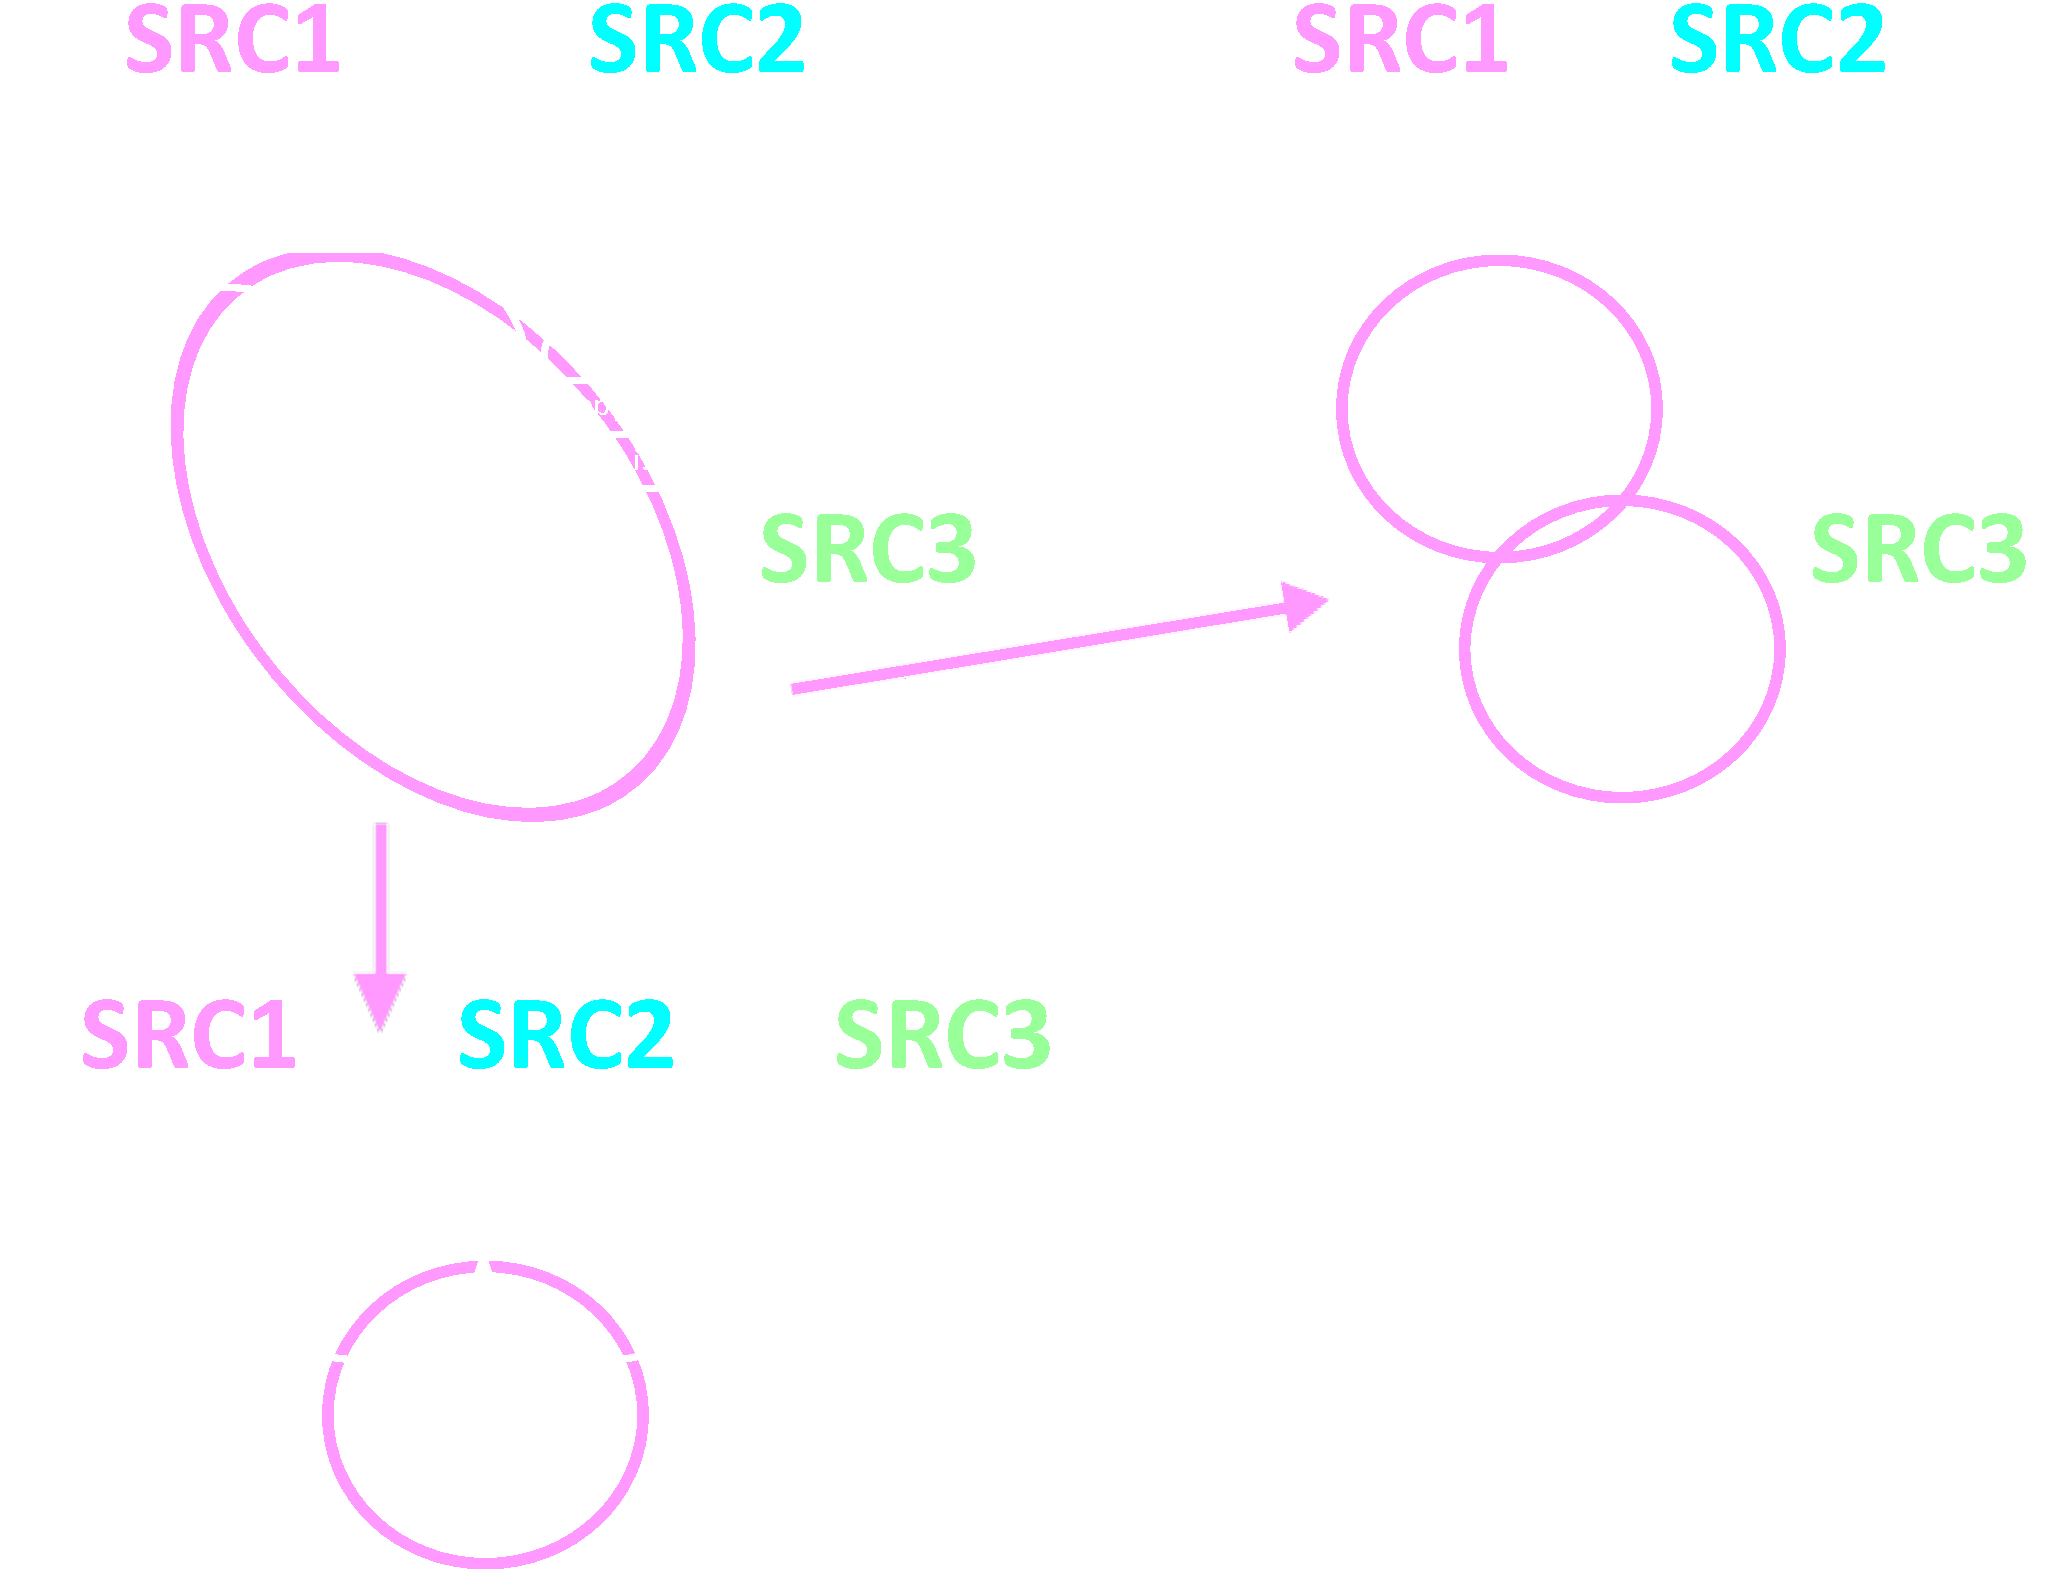
\includegraphics[width = 0.80\textwidth]{examples/ex3/ex3-isel-comparison.pdf}

\end{frame}
